\documentclass{tikzposter}

\usepackage[english]{babel}
\usepackage[utf8]{inputenc}
\usepackage{graphicx}

\usepackage{listings}
\usepackage{xcolor}
\usepackage{tcolorbox}
\lstset{ basicstyle=\ttfamily }
\definecolor{codegray}{rgb}{0.8,0.8,0.8}
\newcommand{\code}[1]{\colorbox{codegray}{\lstinline|#1|}}

\usetheme{Envelope}

\title{Bot Specification Sheet}
\author{dkantereivin, Doomer}
\date{\today}

\begin{document}
    \maketitle
    \begin{columns}
        \column{0.7}
        \block{Introduction}{
            This is the Bot Specification Sheet - here every feature and their usage will
            be documented! The `Short Feature List' offers a run-down on all the general 
            Commands and Events by simply listing them, which can be used to get a quick
            glance over the whole project!\\
            The `Extended Feature List' will provide a small `man'-like entry for each 
            feature, describe how it can be triggered, the passable arguments and the
            result / purpose of the respective feature! The document will assume that 
            `\$' is the prefix, so commands can be illustrated in a better fashion.
        }
        \column{0.3}
        \block{}{
            \begin{center}
                
\includegraphics{img/logo512.png}
            \end{center}
        }
    \end{columns}
    \begin{columns}
        \column{0.3}  % See Section 4.4
        \block{Short Feature List}{
            \textbf{Commands:}

            \begin{itemize}
                \item[$\diamond$] \code{help}-command
                \item[$\diamond$] \code{ping}-command
                \item[$\diamond$] \code{sudo}-command
                \item[$\diamond$] \code{whois}-command
            \end{itemize}

            \textbf{Events:}

            \begin{itemize}
                \item[$\diamond$] \code{ready}-event
                \item[$\diamond$] \code{message}-event
                \item[$\diamond$] \code{messageReactionAdd}-event 
            \end{itemize}

            \textbf{Services:}

            \begin{itemize}
                \item[$\diamond$] \code{config}-service
                \item[$\diamond$] \code{logger}-service
                \item[$\diamond$] \code{rate-limit}-service 
            \end{itemize}
        }
        \block{Screenshots}{
            \textbf{Help Command}:\vspace{0.3cm}\\
            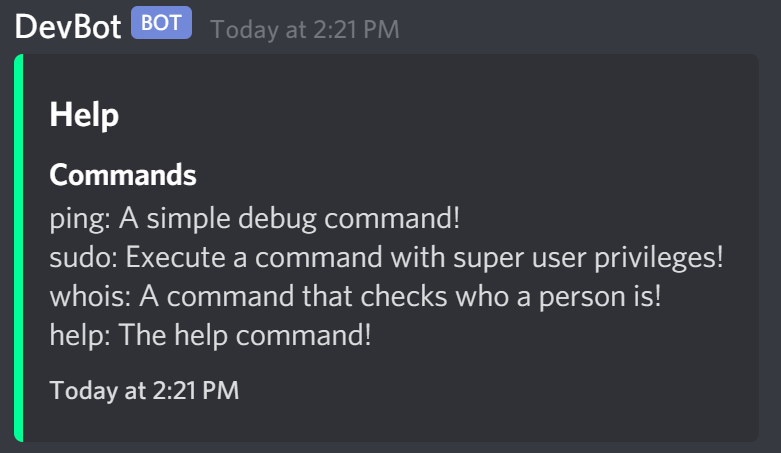
\includegraphics[width=600px]{img/help-snip.png}\\
            \textbf{Who Is Command}:\vspace{0.3cm}\\
            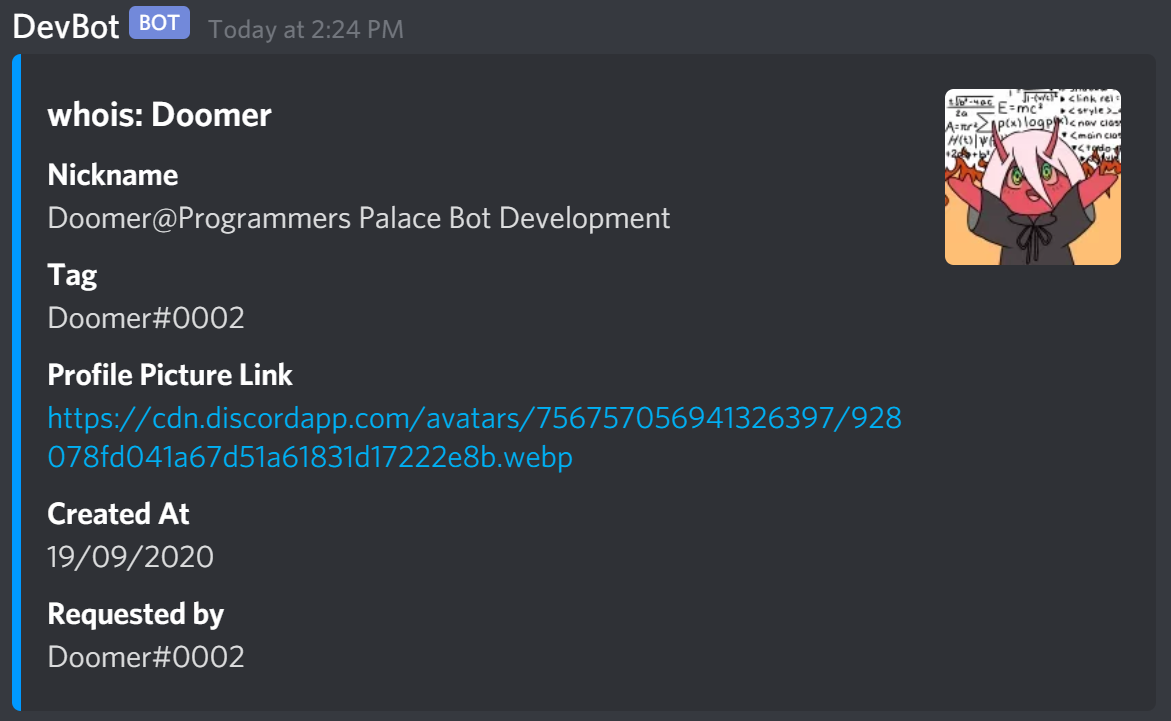
\includegraphics[width=600px]{img/whois-snip.png}
        }
        \column{0.7}
        \block{Extended Feature List}{
            \textbf{Help Command}:\\
            \textit{Purpose:} The help command provides information about the
            currently accessible top-level commands. A short description
            alongside the command name is sent inside an embed to provide a
            general idea of what a command does. The reload flag reloads
            the help message, in order to allow the information to change 
            during runtime in case that new aliases were added!\\
            \textit{Syntax:} \code{\$help [--reload \| --help]}\\
            \textbf{Ping Command}:\\
            \textit{Purpose:} The ping command serves two functions. For the
            developer the ping command is one of the simplest, so it is used
            as a code template for further commands, to showcase the Command
            architecture. The user can use the ping command to detect whether
            the bot is online at the moment or not!\\
            \textit{Syntax:} \code{\$ping [--help]}\\
            \textbf{Sudo Command}:\\
            \textit{Purpose:} The sudo command provides a way to execute 
            commands with super user (a.k.a. Admin) privileges. One could use
            sudo to handle different behaviours of command - depending on 
            whether it was called through \code{sudo} or not! In the future
            this command might obtain more meaning, once the permission system
            is in place!\\
            \textit{Syntax:} \code{\$sudo [--help]} or \code{\$sudo [ping]}\\
            \textbf{Who Is Command}:\\
            \textit{Purpose:} The who is command sends certain information, 
            such as User Tag, Profile Picture, and similar information about
            a user once called! It's `image' flag can be used to only print
            the image of the user and thus - thanks to Discords Link Parsing
            show an image of the Person's Avatar in the Chat!\\
            \textit{Syntax:} \code{\$whois [--image \| --help]}\vspace{2cm}\\
            \textbf{Ready Event}:\\
            \textit{Purpose:} This event gets fired as soon as the Discord
            Bot Client logs onto the network! This Event can be used to 
            setup everything that requires the bot to be online, such as
            cache the prefixes of the servers the bot is in!\\
            \textbf{Message Event}:\\
            \textit{Purpose:} The message event is responsible for receiving
            messages and find commands and other important triggers in them!
            The message event is the base of this whole project, since the bot
            - as expected of a Discord Bot - is mostly controlled through 
            user input on Discord!\\
            \textbf{Message Reaction Add Event}:\\
            \textit{Purpose:} This event occurs when a reaction is added to a 
            message (note: the bot had to be online when the message was sent
            for it to work!). This event is used by this Bot for the Message
            Flagging Mechanic! A message can be flagged using emojis, reviewed
            in a separate channel and upon approval be added into a Database 
            (not yet implemented).\vspace{2cm}\\
            \textbf{Config Service}:\\
            \textit{Purpose:} The config service is used to load the initial
            bot config, such as the bot token and a default prefix! It also 
            stores information such as the Discord Rich Presence!\\
            \textbf{Logger Service}:\\
            \textit{Purpose:} The logger service as one can tell by the name
            exposes a logger to the developer, which can be used to track 
            the state of the bot and collect debug information.\\
            \textbf{Rate Limit Service}:\\
            \textit{Purpose:} The rate limit service is used to limit the rate
            at which commands can get executed by an individual. In future the
            exceeding of the rate limit likely will get logged and suspicious
            behaviour will be reported to the Admins.
        }
    \end{columns}
\end{document}